\documentclass[11pt]{article}
\usepackage{amsmath,amsfonts}
\usepackage[numbers,sort&compress]{natbib}
\usepackage{times}
\usepackage[left=2.54cm,top=2.54cm,right=2.54cm,bottom=2.54cm,bindingoffset=0.0cm]{geometry}
\usepackage{setspace}
\usepackage{enumerate}
\usepackage{enumitem}
\usepackage{wrapfig}
\setcounter{secnumdepth}{0}
\usepackage{fullpage}
\usepackage{titlesec}
\titleformat{\section}{\large\bfseries}{\thesection}{1em}{}
\titleformat{\subsection}{\bfseries}{\thesubsection}{1em}{}
\usepackage{parskip} % skip paragraph indentations
\usepackage{lipsum}
\usepackage{hyperref}
\usepackage{graphicx}
\usepackage{amssymb}
\usepackage[x11names]{xcolor}
\usepackage{hyperref}
\usepackage{enumitem}
\usepackage{booktabs}
\usepackage{amsmath}
\usepackage{amssymb}
\usepackage{mathrsfs}
\usepackage{caption} \captionsetup[table]{singlelinecheck=false} %makes table captions left-justified
\usepackage{framed} % to add frames around comments
%\hypersetup{backref,colorlinks=false,
%    urlbordercolor=LightSkyBlue4,          % color of internal links
%    citebordercolor=SpringGreen4,        % color of links to bibliography
%    filebordercolor=magenta,      % color of file links
%    linkbordercolor=Red3, pdfborderstyle={/S/U/W 1.5}}
\newcommand{\Prob}[1]{\Pr{\left( #1 \right)}}
\newcommand{\q}[1]{``#1''} % easier way to get double quotes
\newcommand{\argmin}{\text{argmin}}
\usepackage{authblk} % for title page
\renewcommand\Affilfont{\fontsize{10}{10.8}\itshape}
\renewcommand\familydefault{\sfdefault} 
\usepackage{datetime2}
%\renewcommand{\dateseparator}{-}
\usepackage{atbegshi}% http://ctan.org/pkg/atbegshi -- removes blank page at start of doc
\AtBeginDocument{\AtBeginShipoutNext{\AtBeginShipoutDiscard}}
\setcounter{page}{0}
\begin{document}
\noindent
\title{Draft: Learned badges vs. Social recognition} 
%The evolution of rank signaling?

\author[1]{Eleanor Brush}
\affil[1]{University of Maryland; email: xxxxx}
\author[2,3]{Elizabeth A. Hobson}
\affil[2]{Santa Fe Institute, 1399 Hyde Park Road, Santa Fe, NM 87501 USA}
\affil[3]{National Institute for Mathematical and Biological Synthesis, University of Tennessee, Knoxville, TN, USA; email: ehobson@nimbios.org}
%\date{} 
\maketitle

%%%%%%%%%%%%%%%%%%%%%%%
\section*{Overview of previous research, outstanding questions, goals} 
%%%%%%%%%%%%%%%%%%%%%%%

Species have different ways of assessing the quality of others. Quality here is used broadly, and can indicate an individual's body condition or immune status, overall reproductive potential, or fitness. Individuals can gain long-term benefits from assessing each others' quality. In the context of conflicts when individuals differ in fighting ability, resource-holding potential, or dominance rank, it may be beneficial for individuals to be able to identify and order individuals by quality. 

% summary of previous research
...Lots of investigation into evolution of 'honest' signaling...  


% summary of our focus for the modeling work (learned badge vs learned recognition) 

Species have different ways of assessing the quality of others. Here, we focus on one type of signal -- the badge of status -- and compare it to a system based on individual recognition. A badge is an arbitrary signal, not directly indicative of fighting ability, where the intensity of the signal correlates with the underlying quality of the individual (here, rank/power) (CITE). Another quality assessment system is a combination recognition/relationship method, where individuals that are able to recognize individuals track their actions and event outcomes to infer quality in the absence of a cue or badge of status (CITE). In both cases, individuals must learn about their opponents in order to assess their quality.

At the two extremes, individuals in a pure badge quality signal system would be completely unable to recognize individuals, and would treat all individuals with similar badge intensities as equivalent; individuals in a pure recognition/relationships based quality system would be completely reliant on remembering an individual's actions, and have no other cues to infer that individual's quality or rank. Binning individuals with similar badge intensities into the same category effectively decreases the functional group size to the number of bins, but also increases noise about quality of each individual. An individual recognition-based system is one in which the number of bins equals the number of individuals in the group.  

Many factors likely affect the accuracy and speed of quality assessment in these two systems. Recent work (\cite{sheehan2016evotradeoff}) provides several predictions but focused on predicting differences in signaling systems comparing an innate quality signal to a social recognition system across different species, not within species (\cite{sheehan2016response}). Here, we use a somewhat different approach: we are interested in two hypothetical systems, where individuals learn to assess quality to others in different ways. 

Our goal is to better understand the conditions under which a badge signal or individual recognition would be favored. We simulated quality assessment through fights among individuals. Each time individuals fight, they are able to assess each other's quality and update their previous opinion about quality. We use two quality assessment methods: (1) Badge signal systems: individuals group others into quality categories based on the intensity of badge signals and (2) Recognition systems: individuals use individual recognition to remember the outcome of events with particular individuals to estimate quality. 

%%%%%%%%%%%%%%%%%%%%%%%
\section*{Conceptual description of model} 
%%%%%%%%%%%%%%%%%%%%%%%

\subsection*{General model conditions}
We use an actor-oriented model design. We form naive groups (composed of individuals who have no knowledge of each other), and they must estimate their own quality and the quality of others. In the experience-only case, individuals can only base these estimates of quality on the fights they have with other individuals. In the observation case, individuals use a combination of their direct experience in fights and their observations of the fights of others to estimate quality. We refer to these estimates of quality as each individuals \q{opinion} of the quality of others. These opinions are iteratively updated as individuals are involved in, or observe, subsequent interactions. 

At each time step, we randomly chose two individuals to \q{fight}. The probability of winning and losing these fights is dependent on the underlying difference in individual quality (VAR, with some stochasticity VAR). Once event outcomes are determined, individuals update their opinions of their own quality and the quality of their opponents, according to EQN. If $a_{ij}(t)$ is $i$'s assessment of $j$ at time $t$, after fighting, 
\begin{equation*}
a_{ij}(t+1)=(1-r)a_{ij}(t)+rq_j+\xi,
\end{equation*}
where $r$ is a parameter describing how much $i$ changes its opinion based on its observation and $\xi$ is drawn from a normal distribution with mean $0$ and standard deviation $\sigma_\text{u}$. If $i$ and $j$ have not fought before so $i$ has no assessment of $j$, then after fighting 
\begin{equation*}
a_{ij}(t+1)=(1-r)b_{i}(t)+rq_j+\xi,
\end{equation*}
where $b_i(t)$ is a baseline opinion of any animal it encounters. Specifically, $b_i(t)$ is drawn from a normal distribution with mean equal to the average quality of the group and small standard deviation. 

% QUESTION: how many simulations were run? EB: 25 simulations.

% describe noise / error
We include error in how individuals recognize or categorize individuals, and in the observation case, we also include error in observation of event outcome. In the badge signal case, individuals may mistakenly categorize individuals into neighboring categories. For example, an individual in Category I may be miscategorized into Category II, with the probability of miscategorization determined by an error parameter (VAR) and the category that an individuals is mistakenly assigned dependent on the distance an individual's quality is from a category bound. In individual recognition, a misidentification occurs at a set rate (VAR). When misidentifications occur, another individual is subbed in at random.  

% describe what we measured
We then measured three aspects of learning: learning curves, learning accuracy, and learning time. Learning curves summarize the mean error in quality assessment across all individual opinions for a single run; summarized learning curves show the global mean of learning curves across multiple runs. Learning accuracy summarizes the each individual's final opinion of the quality of others compared to the actual quality of those individuals. Learning time summarizes the number of fights an individual engaged in (or observed) before reaching a threshold within which the opinion matched the final opinion of quality. Learning accuracy and learning time are summarized for each run and plotted as a function of the parameter values. 


\subsection*{Parameter space}
We investigated how varying several parameters affected the learning curves, learning accuracy, and learning time. We varied group size (n=\{25, 50, 75, 100\}), the group's index strength (the correlation between the badge intensity and underlying quality of individuals, s=\{ADD\}), the memory capabilities of agents, and the total number of fights. For the badge signal system, we also specify the number of bins that individuals use to categorize individuals by quality (b=\{2, 5, 10, 15\}). 

For the recognition/relationship system, we set...% anything extra?


\subsection*{Variables}

\begin {table}[h]
\caption {Description of variables} \label{tab:vars} 
\begin{tabular}{cl}
\toprule
 Variables & Description of variables \\
\midrule
n & number of individuals \\ 
 qi & quality of individual i \\ 
 si & signal of quality / badge of status of individual i \\ 
 li & learning accuracy of individual i (pooled across all j individuals) \\
 Tij & individual i's final opinion of j after x fights (set x fight threshold) \\
 $\hat{T}_i$ & median of (Tij)j \\
 
\bottomrule
\end{tabular}
\end {table}

\subsection*{Defining categories}
\textbf{Email text: }I noticed at the end of the day yesterday that since I've changed how the categories are created, for a given perception window, there are fewer categories when signal and quality are poorly correlated, i.e. holding perception window constant but varying correlation changes the number of categories the animals perceive. I'll explain why this happened below if you care, but I've rewritten the code so that varying correlation doesn't affect the number of categories being perceived. It's better because we can only identify the effects of the signal-quality correlation and the perception abilities if they're independent parameters. Since all the lines in the summary plots hold correlation constant, so it shouldn't change any results. 

The issue was in how I generated signal values: First, I draw quality values from a normal distribution. Then, I draw signal values from a normal distribution and rotate them so that the signal values have the desired correlation with the quality values. The way I was rotating kind of squashed the signal values together when correlation was low and spread them out when correlation was high. This didn't matter when we were using number of categories as a parameter because we'd just divvy up the group into that many categories. However, using a perception window, the more similar the animals are, the fewer categories they get binned into, so low correlation meant few categories. I've rewritten how the signal values are generated so that there is more or less the same amount of variation regardless of the quality-signal correlation.

\textbf{Email text: }I reran all the simulations with a new-and-improved way of fixing the correlation between quality and signal and generated new figures. They are, with the exception of running slightly fewer parameters for the sake of time, pretty much identical to the old. I left the old ones in the Dropbox folder just so you could compare and they have "old" at the end of the filename. Figures without "old" are good to go.

"Categories.pdf" is an example of how 25 animals might be categorized when the perception window is 0.3.

"numberofcategories.pdf" shows how the number of categories the group gets divided into depends on the perception window and the group size, in case you'd like to see.

\subsection*{learning times}

\textbf{Email text:} Re: learning time: Within one simulation of one group, I calculate an animal's learning time as the average number of fights it takes to decrease the error in its assessment about each other animal below a threshold, right now, 0.2. For each combination of parameters, I average this learning time across all individuals and all 25 simulations. This is indeed a little different than the first version of the model, where I calculated learning time as the number of fights it takes for error to get within a threshold of its final error, which doesn't make as much sense.

\textbf{Email text: }I got to wondering why learning time is much higher for individual learning when the perception window is 0, since both individual and categorical learners can identify all individuals in the group. I meant to have the probability of confusion be 0 for both types of learning, but I realized that the parameter I've been using  for categorical learning actually allowed for a small probability of two individuals being put in the same category. This means that, if an animal encounters and learns about another animal, there is a small probability that it updates its opinion about other animals that are sufficiently similar. This non-zero probability of confusion actually allows categorical learners to learn more quickly. That to me is a potentially interesting result. BUT for the moment, I'm rerunning simulations where both types of learning have 0 probability of confusion. When I get the chance, I'm planning on a more systematic sweep of the confusion probabilities to see what their effects are. If you use the current figures and someone asks why individual learning takes longer, that's why, and I'll get new figures to you as soon as I can.

\textbf{Email text:} Within one simulation of one group, each animal has an assessment about every other animal at each point in time (it may be NA). Its error about each other animal at each point in time is the absolute difference between that assessment and each other animal's quality (if the assessment is NA, the error is NA). An animal's learning time about each other animal is the number of fights before its error drops below 0.2. Error fluctuates because the animals forget and because there's some noise in every assessment they make. Even though i's error about j dropped below 0.2, it might go back up again. And just because i's error about j is below 0.2, its error about other animals might still be high. So its average error about every other animal might be above the threshold, even while its error about some or all of the other animals has already dropped below the threshold. To generate the learning curves, I take the average of this average error across all individuals and all simulations. So this average can be above the threshold, even while the average learning time is finite. I hope that makes sense. Like I said, a figure illustrating this counterintuitive calculation is on the way. 

\textbf{Email text: } See figure~\ref{learnT.ex}. The parameters are group size = 10, quality to signal correlation = 0.7, perception window = 0.5, memory window = Inf. I ran one simulation of such a group. Then I calculated the error in one animal's assessment of each other animal. There is a squiggly colored line for each of these errors over time. The squiggly black line is the average of these. The horizontal black line is the error threshold. The vertical colored lines are the "learning times" for each animal: the time when the focal animal's error about the other drops below the threshold. The vertical black line is the average of the learning times. The average error remains above the threshold, even though the animal's error about some of the other animals drops below the threshold. I tried to explain this in an earlier email, but it helps me to visualize it, hence the figure.

%%%%%%%%%%%% explanation figures

\begin{figure}[h]
\caption{\sffamily\small\textbf{Categories.}
     xxxxxxx.}
\label{cats_ex}
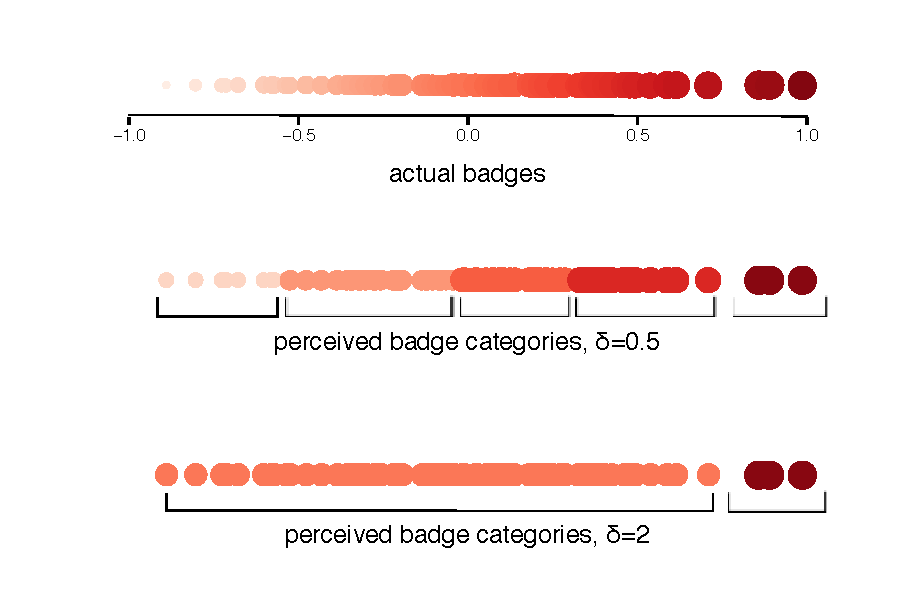
\includegraphics[width=.8\textwidth]{figures/categories.pdf}
\end{figure}

\begin{figure}[h]
\caption{\sffamily\small\textbf{Learning time example.}
     xxx.}
\label{learnT.ex}
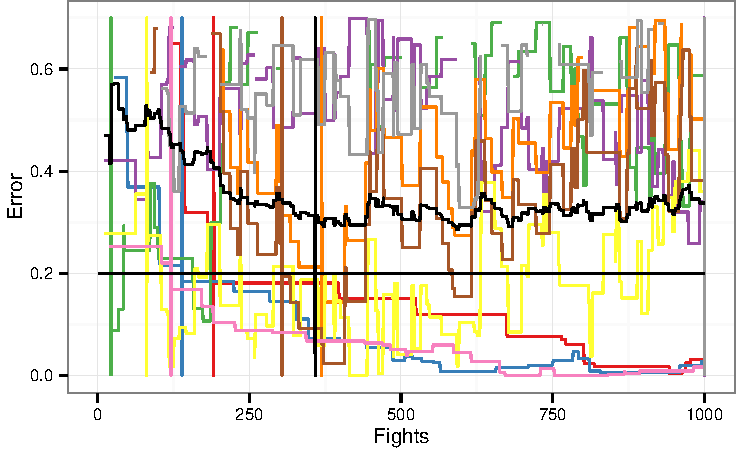
\includegraphics[width=.8\textwidth]{figures/learning_time_example.pdf}
\end{figure}
%%%%%%%%%%%%%%%%%%%%%%%%%%%

\section*{Results}
\subsection*{General results}
\textbf{Email text: }Red is always categorical learning. Blue is always individual learning. The average-error figures show the average (saturated line) plus or minus the standard deviation (shaded area) across all members of a group across all 25 random initial conditions. The title of each panel gives the group size (N), number of categories (number sign), window size (wind), and correlation between quality and signal (corr). All the parameters I've looked at have the expected effect, e.g. increasing group size makes individual learning more error prone. The effect-of-categor-num figure shows how the average error of categorical learning depends on the number of categories being used, for the parameters given in the title. There's a surprising shape here: the lowest error happens at an intermediate number of categories. I'm not sure why this is happening yet, but it's interesting I think. Finally, the learning-times figures give the frequencies across all individuals and all initial conditions of how long it takes the animal to get its error sufficiently close to its error after 10000 fights. Here, too, all of the parameters I've looked at have expected effects, e.g. increasing group size increases the learning time.


\subsection*{How do category bin sizes affect error and learning time?}

\subsection*{How does group size affect error and learning time?}

\subsection*{How does memory affect error and learning time?}


\begin{figure}[ht]
\caption{\sffamily\small\textbf{Learning curves.}
     Cherry-picked parameter combinations to illustrate how learning curves change under different conditions (summarized below).}
\label{learning_curves}
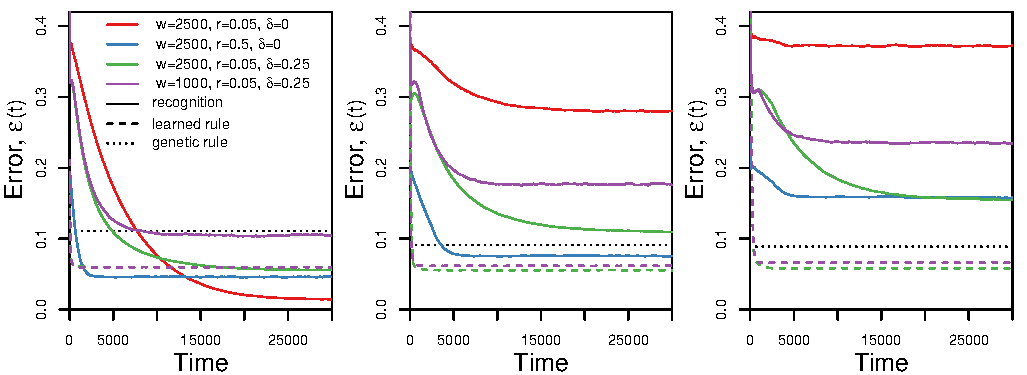
\includegraphics[width=.95\textwidth]{figures/learning_curves.pdf}
\end{figure}

\begin{figure}
\caption{\sffamily\small\textbf{Summary error by group size.}
    xxxxxxx (individualized levels shown for reference).}
\label{summary_error_groupsize}
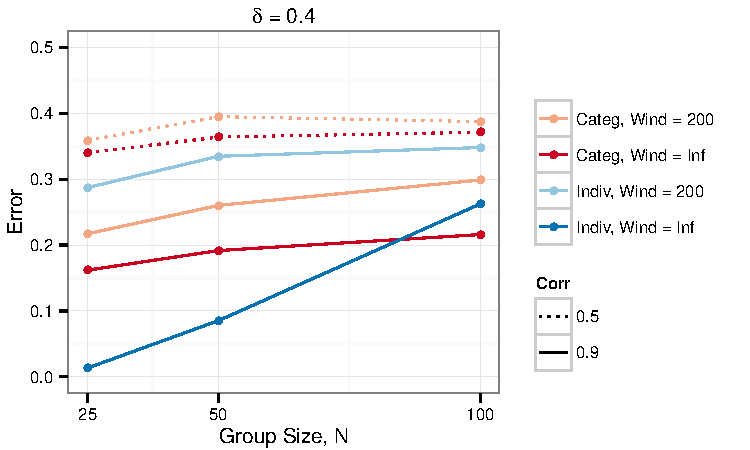
\includegraphics[width=.8\textwidth]{figures/summary_error_groupsize.pdf}
\end{figure}

\begin{figure}
\caption{\sffamily\small\textbf{Summary error by perception window.}
    xxxxxxx (individualized levels shown for reference).}
\label{summary_error}
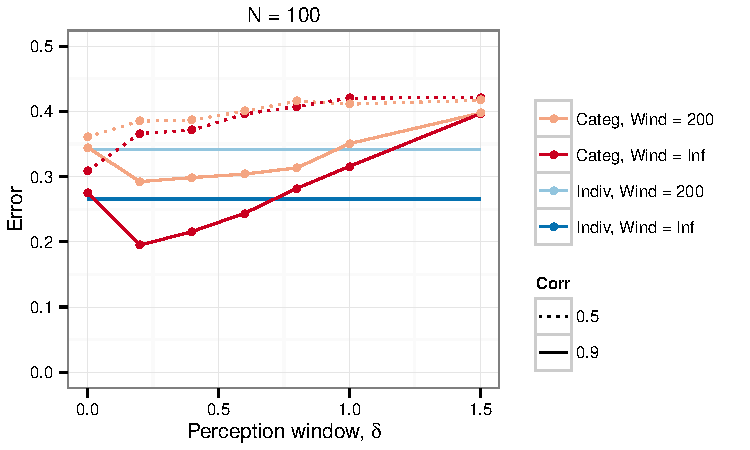
\includegraphics[width=.8\textwidth]{figures/summary_error_percwindow.pdf}
\end{figure}

\begin{figure}
\caption{\sffamily\small\textbf{Summary time by group size.}
     xxxxxxx (individualized levels shown for reference).}
\label{summary_time_groupsize}
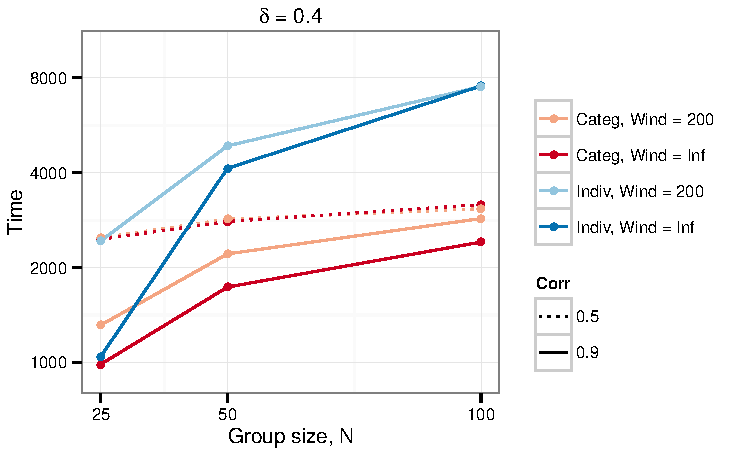
\includegraphics[width=.8\textwidth]{figures/summary_time_groupsize.pdf}
\end{figure}

\begin{figure}
\caption{\sffamily\small\textbf{Summary time by perception window.}
     xxxxxxx (individualized levels shown for reference).}
\label{summary_time_percwindow}
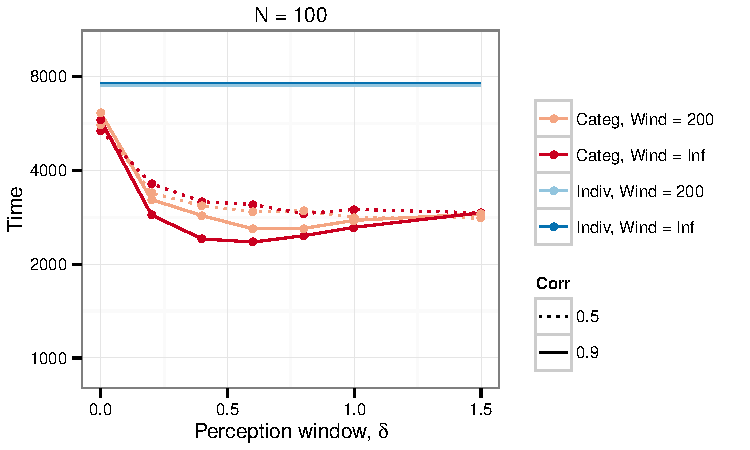
\includegraphics[width=.8\textwidth]{figures/summary_time_percwindow.pdf}
\end{figure}


\newpage
\bibliography{BIB_badgeVSrecog,TODO_newrefs}
\bibliographystyle{apa}

\end{document}

% CUT TEXT

% summary data quantified
We then use the simulated interaction datasets to quantify: 
\begin{enumerate}
  \item Learning curves: each individual's opinion error across the series of fights 
  \item Learning accuracy: amount of error in final opinions about quality (summarize histograms of learning error)
  \item Learning time: amount of fights (time) for opinion to achieve maximum potential accuracy (opinion at end of all fights)  
\end{enumerate}